\documentclass[twoside]{book}

% Packages required by doxygen
\usepackage{fixltx2e}
\usepackage{calc}
\usepackage{doxygen}
\usepackage[export]{adjustbox} % also loads graphicx
\usepackage{graphicx}
\usepackage[utf8]{inputenc}
\usepackage{makeidx}
\usepackage{multicol}
\usepackage{multirow}
\PassOptionsToPackage{warn}{textcomp}
\usepackage{textcomp}
\usepackage[nointegrals]{wasysym}
\usepackage[table]{xcolor}

% Font selection
\usepackage[T1]{fontenc}
\usepackage[scaled=.90]{helvet}
\usepackage{courier}
\usepackage{amssymb}
\usepackage{sectsty}
\renewcommand{\familydefault}{\sfdefault}
\allsectionsfont{%
  \fontseries{bc}\selectfont%
  \color{darkgray}%
}
\renewcommand{\DoxyLabelFont}{%
  \fontseries{bc}\selectfont%
  \color{darkgray}%
}
\newcommand{\+}{\discretionary{\mbox{\scriptsize$\hookleftarrow$}}{}{}}

% Page & text layout
\usepackage{geometry}
\geometry{%
  a4paper,%
  top=2.5cm,%
  bottom=2.5cm,%
  left=2.5cm,%
  right=2.5cm%
}
\tolerance=750
\hfuzz=15pt
\hbadness=750
\setlength{\emergencystretch}{15pt}
\setlength{\parindent}{0cm}
\setlength{\parskip}{3ex plus 2ex minus 2ex}
\makeatletter
\renewcommand{\paragraph}{%
  \@startsection{paragraph}{4}{0ex}{-1.0ex}{1.0ex}{%
    \normalfont\normalsize\bfseries\SS@parafont%
  }%
}
\renewcommand{\subparagraph}{%
  \@startsection{subparagraph}{5}{0ex}{-1.0ex}{1.0ex}{%
    \normalfont\normalsize\bfseries\SS@subparafont%
  }%
}
\makeatother

% Headers & footers
\usepackage{fancyhdr}
\pagestyle{fancyplain}
\fancyhead[LE]{\fancyplain{}{\bfseries\thepage}}
\fancyhead[CE]{\fancyplain{}{}}
\fancyhead[RE]{\fancyplain{}{\bfseries\leftmark}}
\fancyhead[LO]{\fancyplain{}{\bfseries\rightmark}}
\fancyhead[CO]{\fancyplain{}{}}
\fancyhead[RO]{\fancyplain{}{\bfseries\thepage}}
\fancyfoot[LE]{\fancyplain{}{}}
\fancyfoot[CE]{\fancyplain{}{}}
\fancyfoot[RE]{\fancyplain{}{\bfseries\scriptsize Generated by Doxygen }}
\fancyfoot[LO]{\fancyplain{}{\bfseries\scriptsize Generated by Doxygen }}
\fancyfoot[CO]{\fancyplain{}{}}
\fancyfoot[RO]{\fancyplain{}{}}
\renewcommand{\footrulewidth}{0.4pt}
\renewcommand{\chaptermark}[1]{%
  \markboth{#1}{}%
}
\renewcommand{\sectionmark}[1]{%
  \markright{\thesection\ #1}%
}

% Indices & bibliography
\usepackage{natbib}
\usepackage[titles]{tocloft}
\setcounter{tocdepth}{3}
\setcounter{secnumdepth}{5}
\makeindex

% Hyperlinks (required, but should be loaded last)
\usepackage{ifpdf}
\ifpdf
  \usepackage[pdftex,pagebackref=true]{hyperref}
\else
  \usepackage[ps2pdf,pagebackref=true]{hyperref}
\fi
\hypersetup{%
  colorlinks=true,%
  linkcolor=blue,%
  citecolor=blue,%
  unicode%
}

% Custom commands
\newcommand{\clearemptydoublepage}{%
  \newpage{\pagestyle{empty}\cleardoublepage}%
}

\usepackage{caption}
\captionsetup{labelsep=space,justification=centering,font={bf},singlelinecheck=off,skip=4pt,position=top}

%===== C O N T E N T S =====

\begin{document}

% Titlepage & ToC
\hypersetup{pageanchor=false,
             bookmarksnumbered=true,
             pdfencoding=unicode
            }
\pagenumbering{alph}
\begin{titlepage}
\vspace*{7cm}
\begin{center}%
{\Large Raytracer 3D }\\
\vspace*{1cm}
{\large Generated by Doxygen 1.8.12}\\
\end{center}
\end{titlepage}
\clearemptydoublepage
\pagenumbering{roman}
\tableofcontents
\clearemptydoublepage
\pagenumbering{arabic}
\hypersetup{pageanchor=true}

%--- Begin generated contents ---
\chapter{Class Index}
\section{Class List}
Here are the classes, structs, unions and interfaces with brief descriptions\+:\begin{DoxyCompactList}
\item\contentsline{section}{\hyperlink{class_blade__surface}{Blade\+\_\+surface} }{\pageref{class_blade__surface}}{}
\item\contentsline{section}{\hyperlink{class_bounding__box}{Bounding\+\_\+box} }{\pageref{class_bounding__box}}{}
\item\contentsline{section}{\hyperlink{class_point3_d}{Point3D} }{\pageref{class_point3_d}}{}
\item\contentsline{section}{\hyperlink{class_ray3_d}{Ray3D} }{\pageref{class_ray3_d}}{}
\item\contentsline{section}{\hyperlink{class_receiver}{Receiver} }{\pageref{class_receiver}}{}
\item\contentsline{section}{\hyperlink{class_rib}{Rib} }{\pageref{class_rib}}{}
\item\contentsline{section}{\hyperlink{class_rotor}{Rotor} }{\pageref{class_rotor}}{}
\item\contentsline{section}{\hyperlink{class_scene}{Scene} }{\pageref{class_scene}}{}
\item\contentsline{section}{\hyperlink{class_sphere}{Sphere} }{\pageref{class_sphere}}{}
\item\contentsline{section}{\hyperlink{class_transmitter}{Transmitter} }{\pageref{class_transmitter}}{}
\item\contentsline{section}{\hyperlink{class_triangle}{Triangle} }{\pageref{class_triangle}}{}
\item\contentsline{section}{\hyperlink{class_vector3_d}{Vector3D} }{\pageref{class_vector3_d}}{}
\end{DoxyCompactList}

\chapter{Class Documentation}
\hypertarget{class_blade__surface}{}\section{Blade\+\_\+surface Class Reference}
\label{class_blade__surface}\index{Blade\+\_\+surface@{Blade\+\_\+surface}}


Collaboration diagram for Blade\+\_\+surface\+:
\nopagebreak
\begin{figure}[H]
\begin{center}
\leavevmode
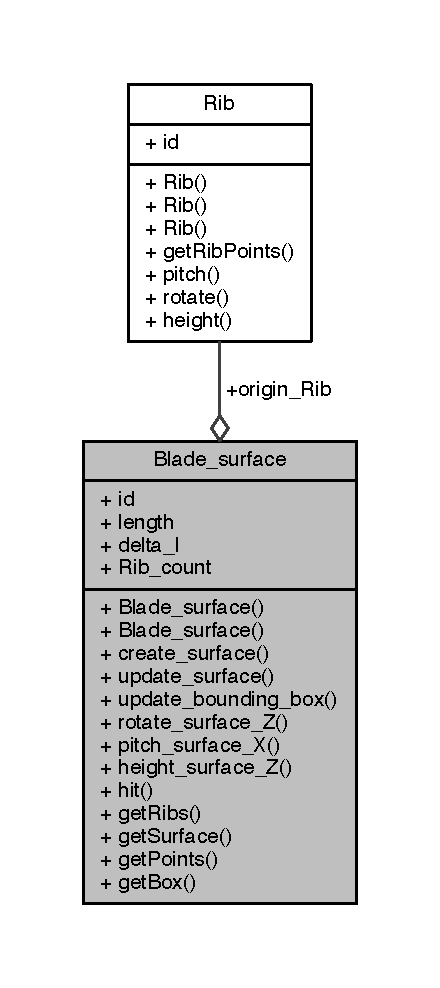
\includegraphics[width=211pt]{doxygen/latex/class_blade__surface__coll__graph}
\end{center}
\end{figure}
\subsection*{Public Member Functions}
\begin{DoxyCompactItemize}
\item 
\hypertarget{class_blade__surface_a0c1a5fa3ea94afa451043ce70d3d7c1e}{}\label{class_blade__surface_a0c1a5fa3ea94afa451043ce70d3d7c1e} 
{\bfseries Blade\+\_\+surface} (const int id, const double length, const int Rib\+\_\+count, \hyperlink{class_rib}{Rib} \&origin\+\_\+\+Rib)
\item 
\hypertarget{class_blade__surface_a160959f632ad73eff846aeea81aa84ae}{}\label{class_blade__surface_a160959f632ad73eff846aeea81aa84ae} 
void {\bfseries create\+\_\+surface} ()
\item 
\hypertarget{class_blade__surface_a34d1f584602a5513960b0647a337232b}{}\label{class_blade__surface_a34d1f584602a5513960b0647a337232b} 
void {\bfseries update\+\_\+surface} ()
\item 
\hypertarget{class_blade__surface_a1eddf9a97aa9c2f4f399d03623e9fb6c}{}\label{class_blade__surface_a1eddf9a97aa9c2f4f399d03623e9fb6c} 
void {\bfseries update\+\_\+bounding\+\_\+box} ()
\item 
\hypertarget{class_blade__surface_a8d08aa093ce9eb861d5061303cc35a3b}{}\label{class_blade__surface_a8d08aa093ce9eb861d5061303cc35a3b} 
void {\bfseries rotate\+\_\+surface\+\_\+Z} (double angle)
\item 
\hypertarget{class_blade__surface_a384b9627c130a436d944264fb001d25b}{}\label{class_blade__surface_a384b9627c130a436d944264fb001d25b} 
void {\bfseries pitch\+\_\+surface\+\_\+X} (const double angle)
\item 
\hypertarget{class_blade__surface_a6823c31d12449828939ddc88ddb23705}{}\label{class_blade__surface_a6823c31d12449828939ddc88ddb23705} 
void {\bfseries height\+\_\+surface\+\_\+Z} (const double height)
\item 
\hypertarget{class_blade__surface_a1d4bc10f18e1ee2002a3fa1b5b0c0cb7}{}\label{class_blade__surface_a1d4bc10f18e1ee2002a3fa1b5b0c0cb7} 
bool {\bfseries hit} (const \hyperlink{class_ray3_d}{Ray3D} \&ray, double \&hit\+Distance, \hyperlink{class_vector3_d}{Vector3D} \&hit\+Normal, \hyperlink{class_point3_d}{Point3D} \&hit\+Point)
\item 
\hypertarget{class_blade__surface_a9d55669ccf429e408ff492cfecf52b6b}{}\label{class_blade__surface_a9d55669ccf429e408ff492cfecf52b6b} 
std\+::vector$<$ \hyperlink{class_rib}{Rib} $>$ {\bfseries get\+Ribs} ()
\item 
\hypertarget{class_blade__surface_a91f5bbe72574182ee6ad9e4014bfebbf}{}\label{class_blade__surface_a91f5bbe72574182ee6ad9e4014bfebbf} 
std\+::vector$<$ \hyperlink{class_triangle}{Triangle} $>$ {\bfseries get\+Surface} ()
\item 
\hypertarget{class_blade__surface_ae2f4aa670e4d320d63c77feffb953ae0}{}\label{class_blade__surface_ae2f4aa670e4d320d63c77feffb953ae0} 
std\+::vector$<$ \hyperlink{class_point3_d}{Point3D} $>$ {\bfseries get\+Points} ()
\item 
\hypertarget{class_blade__surface_a72fcd5b6eeb88c4e18da0ad267b27a93}{}\label{class_blade__surface_a72fcd5b6eeb88c4e18da0ad267b27a93} 
\hyperlink{class_bounding__box}{Bounding\+\_\+box} {\bfseries get\+Box} ()
\end{DoxyCompactItemize}
\subsection*{Public Attributes}
\begin{DoxyCompactItemize}
\item 
\hypertarget{class_blade__surface_afd3c87a82f107470cea4d3c8c1f5ee78}{}\label{class_blade__surface_afd3c87a82f107470cea4d3c8c1f5ee78} 
int {\bfseries id}
\item 
\hypertarget{class_blade__surface_a23f1ef284f842b523cb4b44235c0cdd7}{}\label{class_blade__surface_a23f1ef284f842b523cb4b44235c0cdd7} 
double {\bfseries length}
\item 
\hypertarget{class_blade__surface_ab1e364b4402fa787dea7d3b601e33778}{}\label{class_blade__surface_ab1e364b4402fa787dea7d3b601e33778} 
double {\bfseries delta\+\_\+l}
\item 
\hypertarget{class_blade__surface_a9ff7e20545a1fbb7ad84b00adb35f070}{}\label{class_blade__surface_a9ff7e20545a1fbb7ad84b00adb35f070} 
int {\bfseries Rib\+\_\+count}
\item 
\hypertarget{class_blade__surface_af1982ac4bb6460c4bae24868bd93e8d5}{}\label{class_blade__surface_af1982ac4bb6460c4bae24868bd93e8d5} 
\hyperlink{class_rib}{Rib} {\bfseries origin\+\_\+\+Rib}
\end{DoxyCompactItemize}


The documentation for this class was generated from the following files\+:\begin{DoxyCompactItemize}
\item 
Raytracer3\+D/\+Raytracer3\+D/Blade\+\_\+surface.\+hpp\item 
Raytracer3\+D/\+Raytracer3\+D/Blade\+\_\+surface.\+cpp\end{DoxyCompactItemize}

\hypertarget{class_bounding__box}{}\section{Bounding\+\_\+box Class Reference}
\label{class_bounding__box}\index{Bounding\+\_\+box@{Bounding\+\_\+box}}


Collaboration diagram for Bounding\+\_\+box\+:
\nopagebreak
\begin{figure}[H]
\begin{center}
\leavevmode
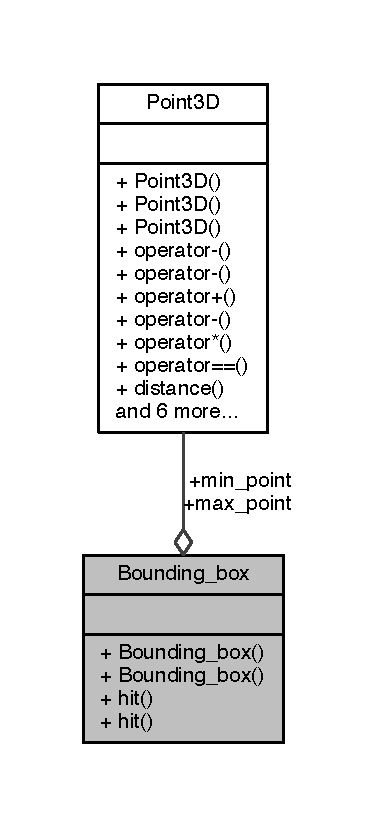
\includegraphics[width=180pt]{doxygen/latex/class_bounding__box__coll__graph}
\end{center}
\end{figure}
\subsection*{Public Member Functions}
\begin{DoxyCompactItemize}
\item 
\hypertarget{class_bounding__box_adf45c090850ee7b48b59f8e586450ef3}{}\label{class_bounding__box_adf45c090850ee7b48b59f8e586450ef3} 
{\bfseries Bounding\+\_\+box} (std\+::vector$<$ \hyperlink{class_point3_d}{Point3D} $>$ \&points)
\item 
\hypertarget{class_bounding__box_a29a6d043ac2de9fb152f39c1139e42df}{}\label{class_bounding__box_a29a6d043ac2de9fb152f39c1139e42df} 
bool {\bfseries hit} (const \hyperlink{class_ray3_d}{Ray3D} \&ray, \hyperlink{class_point3_d}{Point3D} \&hit\+\_\+point) const
\item 
\hypertarget{class_bounding__box_af2a1aa9cee9c82c2dd2df602cca9f42f}{}\label{class_bounding__box_af2a1aa9cee9c82c2dd2df602cca9f42f} 
bool {\bfseries hit} (const \hyperlink{class_ray3_d}{Ray3D} \&ray) const
\end{DoxyCompactItemize}
\subsection*{Public Attributes}
\begin{DoxyCompactItemize}
\item 
\hypertarget{class_bounding__box_add720cf740129c859bddbbed01727c48}{}\label{class_bounding__box_add720cf740129c859bddbbed01727c48} 
\hyperlink{class_point3_d}{Point3D} {\bfseries min\+\_\+point}
\item 
\hypertarget{class_bounding__box_a1ee058e226dbf771065c67d62cac8c66}{}\label{class_bounding__box_a1ee058e226dbf771065c67d62cac8c66} 
\hyperlink{class_point3_d}{Point3D} {\bfseries max\+\_\+point}
\end{DoxyCompactItemize}


The documentation for this class was generated from the following files\+:\begin{DoxyCompactItemize}
\item 
Raytracer3\+D/\+Raytracer3\+D/Bounding\+\_\+box.\+hpp\item 
Raytracer3\+D/\+Raytracer3\+D/Bounding\+\_\+box.\+cpp\end{DoxyCompactItemize}

\hypertarget{class_point3_d}{}\section{Point3D Class Reference}
\label{class_point3_d}\index{Point3D@{Point3D}}


Collaboration diagram for Point3D\+:
\nopagebreak
\begin{figure}[H]
\begin{center}
\leavevmode
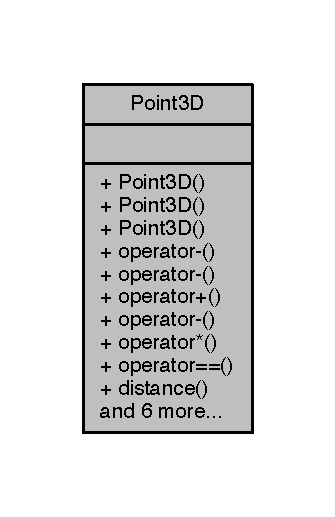
\includegraphics[width=161pt]{doxygen/latex/class_point3_d__coll__graph}
\end{center}
\end{figure}
\subsection*{Public Member Functions}
\begin{DoxyCompactItemize}
\item 
\hypertarget{class_point3_d_a72799f11be08ba98bb37cfcf2fa0bb1f}{}\label{class_point3_d_a72799f11be08ba98bb37cfcf2fa0bb1f} 
{\bfseries Point3D} (const double x, const double y, const double z)
\item 
\hypertarget{class_point3_d_af963fbdffd449c8fc2d0631992a996e1}{}\label{class_point3_d_af963fbdffd449c8fc2d0631992a996e1} 
{\bfseries Point3D} (const double y, const double z)
\item 
\hypertarget{class_point3_d_a7ac9d9c06fe0497d868537d2f6ad9454}{}\label{class_point3_d_a7ac9d9c06fe0497d868537d2f6ad9454} 
\hyperlink{class_point3_d}{Point3D} {\bfseries operator-\/} () const
\item 
\hypertarget{class_point3_d_a6cb0fe83bc148a42fb2cf6f9aa907242}{}\label{class_point3_d_a6cb0fe83bc148a42fb2cf6f9aa907242} 
\hyperlink{class_vector3_d}{Vector3D} {\bfseries operator-\/} (const \hyperlink{class_point3_d}{Point3D} \&p) const
\item 
\hypertarget{class_point3_d_a2ab1c2f322e1845e94414fab67139667}{}\label{class_point3_d_a2ab1c2f322e1845e94414fab67139667} 
\hyperlink{class_point3_d}{Point3D} {\bfseries operator+} (const \hyperlink{class_vector3_d}{Vector3D} \&v) const
\item 
\hypertarget{class_point3_d_a376bb34529614f69a1d79b9633b6ab03}{}\label{class_point3_d_a376bb34529614f69a1d79b9633b6ab03} 
\hyperlink{class_point3_d}{Point3D} {\bfseries operator-\/} (const \hyperlink{class_vector3_d}{Vector3D} \&v) const
\item 
\hypertarget{class_point3_d_a30f07cec680e5e619289ba0c36c00d34}{}\label{class_point3_d_a30f07cec680e5e619289ba0c36c00d34} 
\hyperlink{class_point3_d}{Point3D} {\bfseries operator$\ast$} (const double a) const
\item 
\hypertarget{class_point3_d_a80016919138ae619c4ae603e0c963460}{}\label{class_point3_d_a80016919138ae619c4ae603e0c963460} 
bool {\bfseries operator==} (const \hyperlink{class_point3_d}{Point3D} \&p) const
\item 
\hypertarget{class_point3_d_a3db617345c47ecf25cee2d8bb08712dc}{}\label{class_point3_d_a3db617345c47ecf25cee2d8bb08712dc} 
double {\bfseries distance} (const \hyperlink{class_point3_d}{Point3D} \&p) const
\item 
\hypertarget{class_point3_d_aa2c65a74cd2605f2f46cd7fa88ed537c}{}\label{class_point3_d_aa2c65a74cd2605f2f46cd7fa88ed537c} 
double {\bfseries x} () const
\item 
\hypertarget{class_point3_d_aeeea1fe4bd6b56727b50c569b71f8207}{}\label{class_point3_d_aeeea1fe4bd6b56727b50c569b71f8207} 
double {\bfseries y} () const
\item 
\hypertarget{class_point3_d_ad663c810a730a64d1e000e366fc366ea}{}\label{class_point3_d_ad663c810a730a64d1e000e366fc366ea} 
double {\bfseries z} () const
\item 
\hypertarget{class_point3_d_a02de7d72811aef8bfc6660dd99267682}{}\label{class_point3_d_a02de7d72811aef8bfc6660dd99267682} 
void {\bfseries rotate\+\_\+Z} (const double angle)
\item 
\hypertarget{class_point3_d_aa282f1dc3a75839d0581583f89eeb1ea}{}\label{class_point3_d_aa282f1dc3a75839d0581583f89eeb1ea} 
void {\bfseries rotate\+\_\+X} (const double angle)
\item 
\hypertarget{class_point3_d_af415dc7a082ad664812b02df15902217}{}\label{class_point3_d_af415dc7a082ad664812b02df15902217} 
void {\bfseries translate\+\_\+Z} (const double height)
\end{DoxyCompactItemize}
\subsection*{Friends}
\begin{DoxyCompactItemize}
\item 
\hypertarget{class_point3_d_a84c3d7aa704e44e7f6cfbfe0cb6528f7}{}\label{class_point3_d_a84c3d7aa704e44e7f6cfbfe0cb6528f7} 
void {\bfseries swap} (\hyperlink{class_point3_d}{Point3D} \&a, \hyperlink{class_point3_d}{Point3D} \&b)
\end{DoxyCompactItemize}


The documentation for this class was generated from the following files\+:\begin{DoxyCompactItemize}
\item 
Raytracer3\+D/\+Raytracer3\+D/Point3d.\+hpp\item 
Raytracer3\+D/\+Raytracer3\+D/Point3d.\+cpp\end{DoxyCompactItemize}

\hypertarget{class_ray3_d}{}\section{Ray3D Class Reference}
\label{class_ray3_d}\index{Ray3D@{Ray3D}}


Collaboration diagram for Ray3D\+:
\nopagebreak
\begin{figure}[H]
\begin{center}
\leavevmode
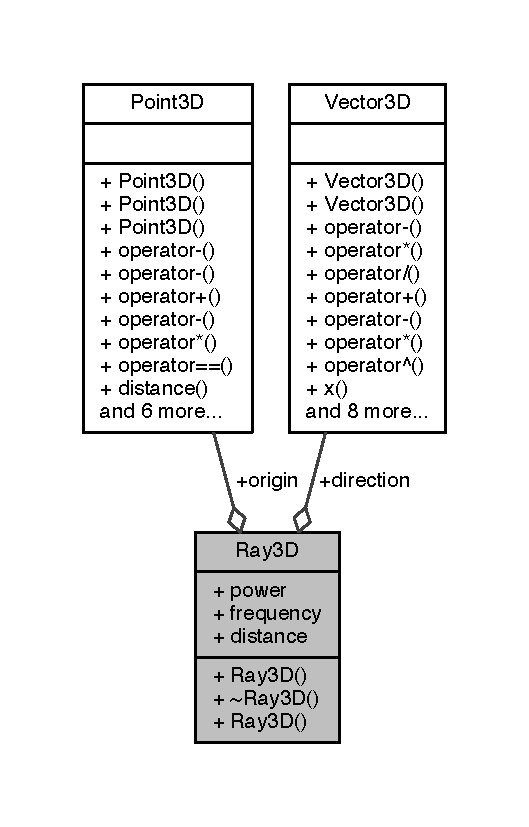
\includegraphics[width=254pt]{doxygen/latex/class_ray3_d__coll__graph}
\end{center}
\end{figure}
\subsection*{Public Member Functions}
\begin{DoxyCompactItemize}
\item 
\hypertarget{class_ray3_d_a0cd2092288763fc6c0fd8dccebf11527}{}\label{class_ray3_d_a0cd2092288763fc6c0fd8dccebf11527} 
{\bfseries Ray3D} (const \hyperlink{class_point3_d}{Point3D} \&origin, const \hyperlink{class_vector3_d}{Vector3D} \&direction, const double power=1.\+0, const double frequency=0.\+0, const double distance=0)
\end{DoxyCompactItemize}
\subsection*{Public Attributes}
\begin{DoxyCompactItemize}
\item 
\hypertarget{class_ray3_d_aa303389d0d8e8569f4bdef420e850717}{}\label{class_ray3_d_aa303389d0d8e8569f4bdef420e850717} 
\hyperlink{class_point3_d}{Point3D} {\bfseries origin}
\item 
\hypertarget{class_ray3_d_a1b9fbe26d23a38f12be002d0e5990fd2}{}\label{class_ray3_d_a1b9fbe26d23a38f12be002d0e5990fd2} 
\hyperlink{class_vector3_d}{Vector3D} {\bfseries direction}
\item 
\hypertarget{class_ray3_d_adbe652ae6043219a7a6d22c3e6a454db}{}\label{class_ray3_d_adbe652ae6043219a7a6d22c3e6a454db} 
double {\bfseries power}
\item 
\hypertarget{class_ray3_d_a5be97a26ac4f733fee0b9a10ca78197a}{}\label{class_ray3_d_a5be97a26ac4f733fee0b9a10ca78197a} 
double {\bfseries frequency}
\item 
\hypertarget{class_ray3_d_a1287339cd3f7358590b2fb65dbb88505}{}\label{class_ray3_d_a1287339cd3f7358590b2fb65dbb88505} 
double {\bfseries distance}
\end{DoxyCompactItemize}


The documentation for this class was generated from the following files\+:\begin{DoxyCompactItemize}
\item 
Raytracer3\+D/\+Raytracer3\+D/Ray3d.\+hpp\item 
Raytracer3\+D/\+Raytracer3\+D/Ray3d.\+cpp\end{DoxyCompactItemize}

\hypertarget{class_receiver}{}\section{Receiver Class Reference}
\label{class_receiver}\index{Receiver@{Receiver}}


Collaboration diagram for Receiver\+:
\nopagebreak
\begin{figure}[H]
\begin{center}
\leavevmode
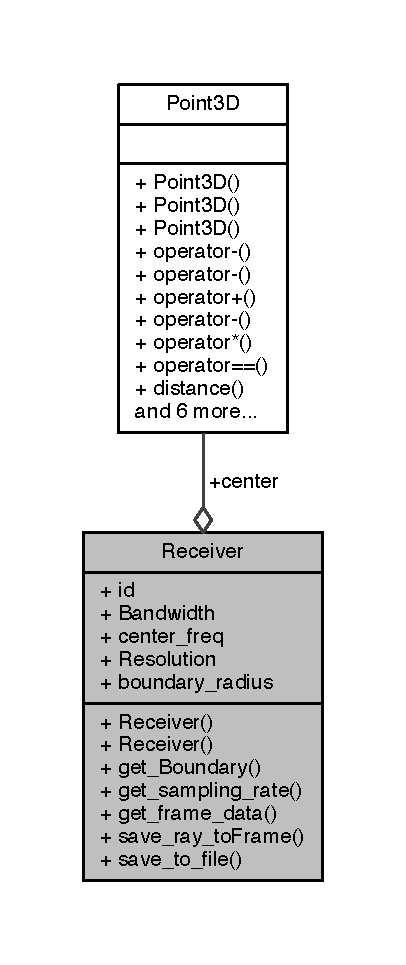
\includegraphics[width=195pt]{doxygen/latex/class_receiver__coll__graph}
\end{center}
\end{figure}
\subsection*{Public Member Functions}
\begin{DoxyCompactItemize}
\item 
\hypertarget{class_receiver_a94a089e687b5320f02b3000304ffd08c}{}\label{class_receiver_a94a089e687b5320f02b3000304ffd08c} 
{\bfseries Receiver} (const int id, const double Bandwidth, const double center\+\_\+freq, const \hyperlink{class_point3_d}{Point3D} \&center, const double boundary\+\_\+radius, const std\+::string \&savefile\+\_\+name, const std\+::string \&dopplerfile\+\_\+name)
\item 
\hypertarget{class_receiver_a6d0f579d480c7303d8138981e546ff01}{}\label{class_receiver_a6d0f579d480c7303d8138981e546ff01} 
\hyperlink{class_sphere}{Sphere} {\bfseries get\+\_\+\+Boundary} ()
\item 
\hypertarget{class_receiver_a6e97969b694ba385a495bf64f9adc16a}{}\label{class_receiver_a6e97969b694ba385a495bf64f9adc16a} 
double {\bfseries get\+\_\+sampling\+\_\+rate} ()
\item 
\hypertarget{class_receiver_a146b5c800df5f2e17eb89faa16a3929a}{}\label{class_receiver_a146b5c800df5f2e17eb89faa16a3929a} 
std\+::vector$<$ \hyperlink{class_ray3_d}{Ray3D} $>$ {\bfseries get\+\_\+frame\+\_\+data} ()
\item 
\hypertarget{class_receiver_aaa3ac7cecd33cba5a382fb0db441082e}{}\label{class_receiver_aaa3ac7cecd33cba5a382fb0db441082e} 
void {\bfseries save\+\_\+ray\+\_\+to\+Frame} (\hyperlink{class_ray3_d}{Ray3D} \&ray)
\item 
\hypertarget{class_receiver_a72ce8129ebd0720a810959eb0a47dfc8}{}\label{class_receiver_a72ce8129ebd0720a810959eb0a47dfc8} 
void {\bfseries save\+\_\+to\+\_\+file} ()
\end{DoxyCompactItemize}
\subsection*{Public Attributes}
\begin{DoxyCompactItemize}
\item 
\hypertarget{class_receiver_aaadfb4436bd66669d03811c846985843}{}\label{class_receiver_aaadfb4436bd66669d03811c846985843} 
int {\bfseries id}
\item 
\hypertarget{class_receiver_a19225a5d1c7c5f4cdaa36b99a1184d26}{}\label{class_receiver_a19225a5d1c7c5f4cdaa36b99a1184d26} 
double {\bfseries Bandwidth}
\item 
\hypertarget{class_receiver_a33f4396a9edddf6fe298108ffa12da58}{}\label{class_receiver_a33f4396a9edddf6fe298108ffa12da58} 
double {\bfseries center\+\_\+freq}
\item 
\hypertarget{class_receiver_a7cf7efbe8c86d8f585e744cbba86c267}{}\label{class_receiver_a7cf7efbe8c86d8f585e744cbba86c267} 
double {\bfseries Resolution}
\item 
\hypertarget{class_receiver_ad9a009e1e386791e5c3bd7211d83a3f9}{}\label{class_receiver_ad9a009e1e386791e5c3bd7211d83a3f9} 
double {\bfseries boundary\+\_\+radius}
\item 
\hypertarget{class_receiver_a4432a9eafa52a2483918d2d3119cb597}{}\label{class_receiver_a4432a9eafa52a2483918d2d3119cb597} 
\hyperlink{class_point3_d}{Point3D} {\bfseries center}
\end{DoxyCompactItemize}


The documentation for this class was generated from the following files\+:\begin{DoxyCompactItemize}
\item 
Raytracer3\+D/\+Raytracer3\+D/Receiver.\+hpp\item 
Raytracer3\+D/\+Raytracer3\+D/Receiver.\+cpp\end{DoxyCompactItemize}

\hypertarget{class_rib}{}\section{Rib Class Reference}
\label{class_rib}\index{Rib@{Rib}}


Collaboration diagram for Rib\+:
\nopagebreak
\begin{figure}[H]
\begin{center}
\leavevmode
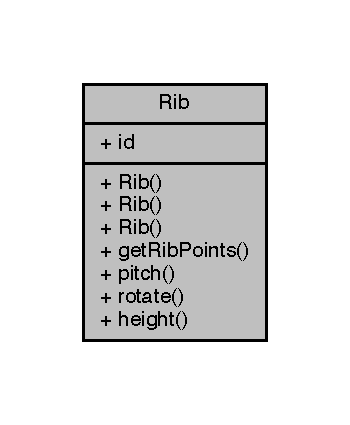
\includegraphics[width=168pt]{doxygen/latex/class_rib__coll__graph}
\end{center}
\end{figure}
\subsection*{Public Member Functions}
\begin{DoxyCompactItemize}
\item 
\hypertarget{class_rib_a417cde052770f55f3344d785aef969ef}{}\label{class_rib_a417cde052770f55f3344d785aef969ef} 
{\bfseries Rib} (int id, \hyperlink{class_rib}{Rib} \&x, const double delta\+\_\+l)
\item 
\hypertarget{class_rib_aaaed7a2c960a33e5ac0c510ea7d8881c}{}\label{class_rib_aaaed7a2c960a33e5ac0c510ea7d8881c} 
{\bfseries Rib} (int id, const std\+::string \&filename)
\item 
\hypertarget{class_rib_ae4ea708286531b624f587f22b9416a36}{}\label{class_rib_ae4ea708286531b624f587f22b9416a36} 
std\+::vector$<$ \hyperlink{class_point3_d}{Point3D} $>$ {\bfseries get\+Rib\+Points} ()
\item 
\hypertarget{class_rib_ab6715214f4a43ed51b46a8f42d6f198b}{}\label{class_rib_ab6715214f4a43ed51b46a8f42d6f198b} 
void {\bfseries pitch} (double angle)
\item 
\hypertarget{class_rib_aafef170600416b0e6a86ccb4e8bd4e32}{}\label{class_rib_aafef170600416b0e6a86ccb4e8bd4e32} 
void {\bfseries rotate} (double angle)
\item 
\hypertarget{class_rib_a08859793a4800c7d160d0b494ad39af7}{}\label{class_rib_a08859793a4800c7d160d0b494ad39af7} 
void {\bfseries height} (const double height)
\end{DoxyCompactItemize}
\subsection*{Public Attributes}
\begin{DoxyCompactItemize}
\item 
\hypertarget{class_rib_ac88341591298af4d11837a09b47917d5}{}\label{class_rib_ac88341591298af4d11837a09b47917d5} 
int {\bfseries id}
\end{DoxyCompactItemize}


The documentation for this class was generated from the following files\+:\begin{DoxyCompactItemize}
\item 
Raytracer3\+D/\+Raytracer3\+D/Rib.\+hpp\item 
Raytracer3\+D/\+Raytracer3\+D/Rib.\+cpp\end{DoxyCompactItemize}

\hypertarget{class_rotor}{}\section{Rotor Class Reference}
\label{class_rotor}\index{Rotor@{Rotor}}


Collaboration diagram for Rotor\+:
\nopagebreak
\begin{figure}[H]
\begin{center}
\leavevmode
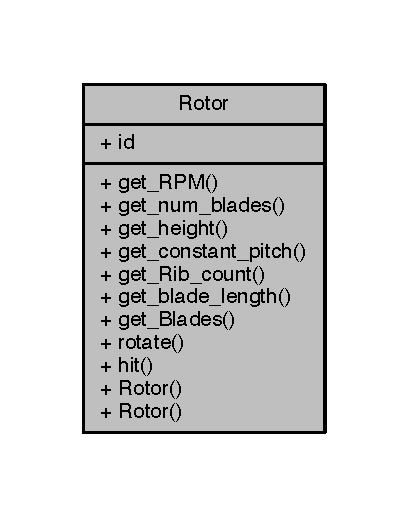
\includegraphics[width=196pt]{doxygen/latex/class_rotor__coll__graph}
\end{center}
\end{figure}
\subsection*{Public Member Functions}
\begin{DoxyCompactItemize}
\item 
\hypertarget{class_rotor_af922b65832291cafdb53c52a545ac136}{}\label{class_rotor_af922b65832291cafdb53c52a545ac136} 
double {\bfseries get\+\_\+\+R\+PM} ()
\item 
\hypertarget{class_rotor_a25eef55d0719b86a255d3aa09f7a2688}{}\label{class_rotor_a25eef55d0719b86a255d3aa09f7a2688} 
int {\bfseries get\+\_\+num\+\_\+blades} ()
\item 
\hypertarget{class_rotor_ad0c276d01564fbdda8ca63c7eff18df6}{}\label{class_rotor_ad0c276d01564fbdda8ca63c7eff18df6} 
double {\bfseries get\+\_\+height} ()
\item 
\hypertarget{class_rotor_a53d18f1d59a1c2b71cdb8c9cab0acd4c}{}\label{class_rotor_a53d18f1d59a1c2b71cdb8c9cab0acd4c} 
double {\bfseries get\+\_\+constant\+\_\+pitch} ()
\item 
\hypertarget{class_rotor_af384431ad8eba046b8541ac5d1a3f9f9}{}\label{class_rotor_af384431ad8eba046b8541ac5d1a3f9f9} 
double {\bfseries get\+\_\+\+Rib\+\_\+count} ()
\item 
\hypertarget{class_rotor_a43485a289837aab864e28dc00109fdf6}{}\label{class_rotor_a43485a289837aab864e28dc00109fdf6} 
double {\bfseries get\+\_\+blade\+\_\+length} ()
\item 
\hypertarget{class_rotor_a31c1b1a9674d87d0b612db4989a4ae16}{}\label{class_rotor_a31c1b1a9674d87d0b612db4989a4ae16} 
std\+::vector$<$ \hyperlink{class_blade__surface}{Blade\+\_\+surface} $>$ {\bfseries get\+\_\+\+Blades} ()
\item 
\hypertarget{class_rotor_ac73f8ab43793bc45b978c6ef14239a4c}{}\label{class_rotor_ac73f8ab43793bc45b978c6ef14239a4c} 
void {\bfseries rotate} (const double angle)
\item 
\hypertarget{class_rotor_ab1ecb2c8efc6e125db1fe9121c6c47b9}{}\label{class_rotor_ab1ecb2c8efc6e125db1fe9121c6c47b9} 
bool {\bfseries hit} (const \hyperlink{class_ray3_d}{Ray3D} \&ray, double \&hit\+Distance, \hyperlink{class_vector3_d}{Vector3D} \&hit\+Normal, \hyperlink{class_point3_d}{Point3D} \&hit\+Point)
\item 
\hypertarget{class_rotor_ad525c69ea4ba137f953675839befcaa6}{}\label{class_rotor_ad525c69ea4ba137f953675839befcaa6} 
{\bfseries Rotor} (const int id, const int num\+\_\+blades, const double R\+PM, const double height, const double constant\+\_\+pitch, const double blade\+\_\+length, const int Rib\+\_\+count)
\end{DoxyCompactItemize}
\subsection*{Public Attributes}
\begin{DoxyCompactItemize}
\item 
\hypertarget{class_rotor_abcb7f6ed3121a0734eef3763d4d20172}{}\label{class_rotor_abcb7f6ed3121a0734eef3763d4d20172} 
int {\bfseries id}
\end{DoxyCompactItemize}


The documentation for this class was generated from the following files\+:\begin{DoxyCompactItemize}
\item 
Raytracer3\+D/\+Raytracer3\+D/Rotor.\+hpp\item 
Raytracer3\+D/\+Raytracer3\+D/Rotor.\+cpp\end{DoxyCompactItemize}

\hypertarget{class_scene}{}\section{Scene Class Reference}
\label{class_scene}\index{Scene@{Scene}}


Collaboration diagram for Scene\+:
\nopagebreak
\begin{figure}[H]
\begin{center}
\leavevmode
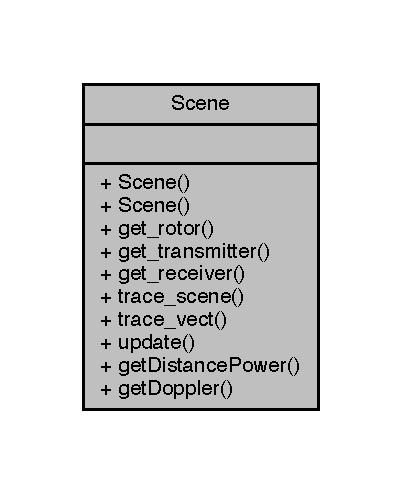
\includegraphics[width=193pt]{doxygen/latex/class_scene__coll__graph}
\end{center}
\end{figure}
\subsection*{Public Member Functions}
\begin{DoxyCompactItemize}
\item 
\hypertarget{class_scene_a39f55da2de994a41500a2c0a3bbc207d}{}\label{class_scene_a39f55da2de994a41500a2c0a3bbc207d} 
{\bfseries Scene} (double rx\+\_\+x, double rx\+\_\+y, double rx\+\_\+z, double Bandwidth, double rx\+\_\+fc, double tx\+\_\+x, double tx\+\_\+y, double tx\+\_\+fc, double tx\+\_\+power, int num\+\_\+blades, double R\+PM, double altitude, double pitch, double blade\+\_\+length, int num\+\_\+ribs, const std\+::string \&filename)
\item 
\hypertarget{class_scene_a59d78e42eebf29106e413275abacf983}{}\label{class_scene_a59d78e42eebf29106e413275abacf983} 
\hyperlink{class_rotor}{Rotor} {\bfseries get\+\_\+rotor} ()
\item 
\hypertarget{class_scene_aeca85b3d6824c3509c94991136fe6a1b}{}\label{class_scene_aeca85b3d6824c3509c94991136fe6a1b} 
\hyperlink{class_transmitter}{Transmitter} {\bfseries get\+\_\+transmitter} ()
\item 
\hypertarget{class_scene_aea609d389de6e5c483d3e7f19a3aff0a}{}\label{class_scene_aea609d389de6e5c483d3e7f19a3aff0a} 
\hyperlink{class_receiver}{Receiver} {\bfseries get\+\_\+receiver} ()
\item 
\hypertarget{class_scene_a2d3012d31a139a597d50f5b84fbec51d}{}\label{class_scene_a2d3012d31a139a597d50f5b84fbec51d} 
void {\bfseries trace\+\_\+scene} (int num\+\_\+rays)
\item 
\hypertarget{class_scene_a26979e16c27d21bdd615c24c1c11902c}{}\label{class_scene_a26979e16c27d21bdd615c24c1c11902c} 
void {\bfseries trace\+\_\+vect} (\hyperlink{class_ray3_d}{Ray3D} \&test\+\_\+ray, double \&hit\+Distance, \hyperlink{class_vector3_d}{Vector3D} \&hit\+Normal, \hyperlink{class_point3_d}{Point3D} \&hit\+Point)
\item 
\hypertarget{class_scene_a9af282cee68bb4748bd15568bda0ecfb}{}\label{class_scene_a9af282cee68bb4748bd15568bda0ecfb} 
void {\bfseries update} (double angle)
\item 
\hypertarget{class_scene_a76fa370d0c210100d4cf8799474faa8d}{}\label{class_scene_a76fa370d0c210100d4cf8799474faa8d} 
double {\bfseries get\+Distance\+Power} (const double frequency, const double power, const double distance) const
\item 
double \hyperlink{class_scene_a969abe0e6022d73ff082d380c59d83f5}{get\+Doppler} (\hyperlink{class_ray3_d}{Ray3D} \&test\+\_\+ray, \hyperlink{class_vector3_d}{Vector3D} \&hit\+Normal, \hyperlink{class_point3_d}{Point3D} \&hit\+Point, double R\+PM) const
\end{DoxyCompactItemize}

The documentation for this class was generated from the following files\+:\begin{DoxyCompactItemize}
\item 
Raytracer3\+D/\+Raytracer3\+D/Scene.\+hpp\item 
Raytracer3\+D/\+Raytracer3\+D/Scene.\+cpp\end{DoxyCompactItemize}

\hypertarget{class_sphere}{}\section{Sphere Class Reference}
\label{class_sphere}\index{Sphere@{Sphere}}


Collaboration diagram for Sphere\+:
\nopagebreak
\begin{figure}[H]
\begin{center}
\leavevmode
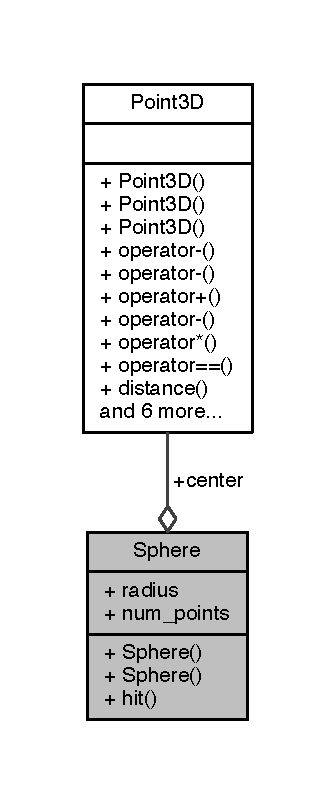
\includegraphics[width=161pt]{doxygen/latex/class_sphere__coll__graph}
\end{center}
\end{figure}
\subsection*{Public Member Functions}
\begin{DoxyCompactItemize}
\item 
\hypertarget{class_sphere_a7b5d0be5fd60ba94573e3941cf4eb094}{}\label{class_sphere_a7b5d0be5fd60ba94573e3941cf4eb094} 
{\bfseries Sphere} (const double radius, const \hyperlink{class_point3_d}{Point3D} \&center)
\item 
\hypertarget{class_sphere_a5da44ddc57c5a68a1092b0df86dc18cd}{}\label{class_sphere_a5da44ddc57c5a68a1092b0df86dc18cd} 
bool {\bfseries hit} (const \hyperlink{class_ray3_d}{Ray3D} \&ray, double \&hit\+Distance, \hyperlink{class_vector3_d}{Vector3D} \&hit\+Normal, \hyperlink{class_point3_d}{Point3D} \&hit\+Point) const
\end{DoxyCompactItemize}
\subsection*{Public Attributes}
\begin{DoxyCompactItemize}
\item 
\hypertarget{class_sphere_a45d6c6c870fac7c2a885ad2e226334ad}{}\label{class_sphere_a45d6c6c870fac7c2a885ad2e226334ad} 
double {\bfseries radius}
\item 
\hypertarget{class_sphere_a774cb90ed1b46592e63a112338f1cc58}{}\label{class_sphere_a774cb90ed1b46592e63a112338f1cc58} 
\hyperlink{class_point3_d}{Point3D} {\bfseries center}
\item 
\hypertarget{class_sphere_a50d3abf7b35058bae9bcbba998a82943}{}\label{class_sphere_a50d3abf7b35058bae9bcbba998a82943} 
int {\bfseries num\+\_\+points}
\end{DoxyCompactItemize}


The documentation for this class was generated from the following files\+:\begin{DoxyCompactItemize}
\item 
Raytracer3\+D/\+Raytracer3\+D/Sphere.\+hpp\item 
Raytracer3\+D/\+Raytracer3\+D/Sphere.\+cpp\end{DoxyCompactItemize}

\hypertarget{class_transmitter}{}\section{Transmitter Class Reference}
\label{class_transmitter}\index{Transmitter@{Transmitter}}


Collaboration diagram for Transmitter\+:
\nopagebreak
\begin{figure}[H]
\begin{center}
\leavevmode
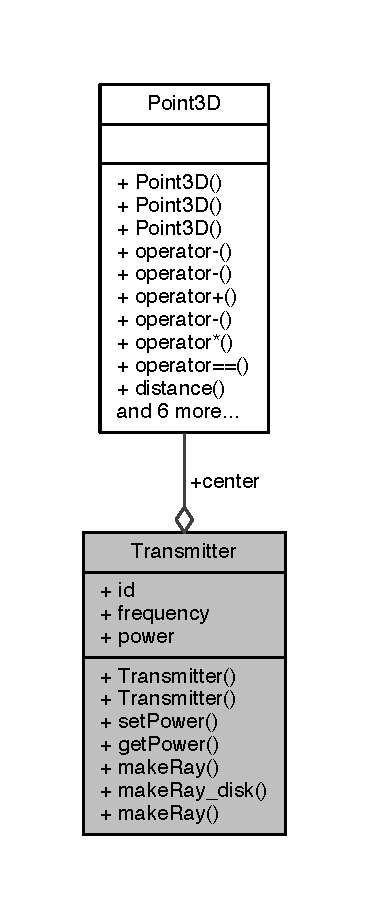
\includegraphics[width=177pt]{doxygen/latex/class_transmitter__coll__graph}
\end{center}
\end{figure}
\subsection*{Public Member Functions}
\begin{DoxyCompactItemize}
\item 
\hypertarget{class_transmitter_a91c51bc1d7c42db81fb390753de5c0ea}{}\label{class_transmitter_a91c51bc1d7c42db81fb390753de5c0ea} 
{\bfseries Transmitter} (const int id, const double frequency, const double power, const \hyperlink{class_point3_d}{Point3D} \&center, const double l)
\item 
\hypertarget{class_transmitter_aa26f745526cba27666812ca7c05b9df7}{}\label{class_transmitter_aa26f745526cba27666812ca7c05b9df7} 
void {\bfseries set\+Power} (const double power)
\item 
\hypertarget{class_transmitter_a72eb7b0c29d6d5e3429f9920dcdf86c9}{}\label{class_transmitter_a72eb7b0c29d6d5e3429f9920dcdf86c9} 
double {\bfseries get\+Power} () const
\item 
\hypertarget{class_transmitter_a8a2727ad1e4b48ec9f64c0285bb5bd04}{}\label{class_transmitter_a8a2727ad1e4b48ec9f64c0285bb5bd04} 
\hyperlink{class_ray3_d}{Ray3D} {\bfseries make\+Ray} ()
\item 
\hypertarget{class_transmitter_a7c51cee738e95fb6f2af955986873b7c}{}\label{class_transmitter_a7c51cee738e95fb6f2af955986873b7c} 
\hyperlink{class_ray3_d}{Ray3D} {\bfseries make\+Ray\+\_\+disk} (const double height)
\item 
\hypertarget{class_transmitter_a5c6bdf0d0dd931f9f4282a7d585f2320}{}\label{class_transmitter_a5c6bdf0d0dd931f9f4282a7d585f2320} 
\hyperlink{class_ray3_d}{Ray3D} {\bfseries make\+Ray} (const \hyperlink{class_vector3_d}{Vector3D} \&ray\+Direction)
\end{DoxyCompactItemize}
\subsection*{Public Attributes}
\begin{DoxyCompactItemize}
\item 
\hypertarget{class_transmitter_a3e57cbedcf7ff80c3506c47d43119f5d}{}\label{class_transmitter_a3e57cbedcf7ff80c3506c47d43119f5d} 
int {\bfseries id}
\item 
\hypertarget{class_transmitter_ade036fee92a7f2aad8ecf206f89b8c34}{}\label{class_transmitter_ade036fee92a7f2aad8ecf206f89b8c34} 
double {\bfseries frequency}
\item 
\hypertarget{class_transmitter_a61c6aa4371c98b49d2d9277fd4447f34}{}\label{class_transmitter_a61c6aa4371c98b49d2d9277fd4447f34} 
\hyperlink{class_point3_d}{Point3D} {\bfseries center}
\item 
\hypertarget{class_transmitter_ac339f9fd3011afdbdc729b99b371e617}{}\label{class_transmitter_ac339f9fd3011afdbdc729b99b371e617} 
double {\bfseries power}
\end{DoxyCompactItemize}


The documentation for this class was generated from the following files\+:\begin{DoxyCompactItemize}
\item 
Raytracer3\+D/\+Raytracer3\+D/Transmitter.\+hpp\item 
Raytracer3\+D/\+Raytracer3\+D/Transmitter.\+cpp\end{DoxyCompactItemize}

\hypertarget{class_triangle}{}\section{Triangle Class Reference}
\label{class_triangle}\index{Triangle@{Triangle}}


Collaboration diagram for Triangle\+:
\nopagebreak
\begin{figure}[H]
\begin{center}
\leavevmode
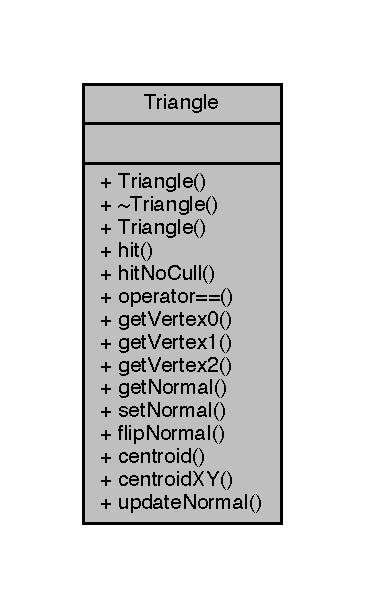
\includegraphics[width=175pt]{doxygen/latex/class_triangle__coll__graph}
\end{center}
\end{figure}
\subsection*{Public Member Functions}
\begin{DoxyCompactItemize}
\item 
\hypertarget{class_triangle_a995e961620da6b595053ef5560999244}{}\label{class_triangle_a995e961620da6b595053ef5560999244} 
{\bfseries Triangle} (\hyperlink{class_point3_d}{Point3D} \&v0, \hyperlink{class_point3_d}{Point3D} \&v1, \hyperlink{class_point3_d}{Point3D} \&v2)
\item 
\hypertarget{class_triangle_ab09716ce6c0928ce11fe34091c19a1c4}{}\label{class_triangle_ab09716ce6c0928ce11fe34091c19a1c4} 
bool {\bfseries hit} (const \hyperlink{class_ray3_d}{Ray3D} \&ray, double \&hit\+Distance, \hyperlink{class_vector3_d}{Vector3D} \&hit\+Normal, \hyperlink{class_point3_d}{Point3D} \&hit\+Point) const
\item 
\hypertarget{class_triangle_a7b93ca1524b80830bf8ea07d660ace6a}{}\label{class_triangle_a7b93ca1524b80830bf8ea07d660ace6a} 
bool {\bfseries hit\+No\+Cull} (const \hyperlink{class_ray3_d}{Ray3D} \&ray, double \&hit\+Distance, \hyperlink{class_vector3_d}{Vector3D} \&hit\+Normal, \hyperlink{class_point3_d}{Point3D} \&hit\+Point) const
\item 
\hypertarget{class_triangle_aeeced29a75e5c27db3457804debbb936}{}\label{class_triangle_aeeced29a75e5c27db3457804debbb936} 
bool {\bfseries operator==} (\hyperlink{class_triangle}{Triangle} \&Tri)
\item 
\hypertarget{class_triangle_a7dbe3b94aae0c1966801d50190ab2c25}{}\label{class_triangle_a7dbe3b94aae0c1966801d50190ab2c25} 
\hyperlink{class_point3_d}{Point3D} {\bfseries get\+Vertex0} ()
\item 
\hypertarget{class_triangle_a88c0bdcbda9d290e7ea876714b634b83}{}\label{class_triangle_a88c0bdcbda9d290e7ea876714b634b83} 
\hyperlink{class_point3_d}{Point3D} {\bfseries get\+Vertex1} ()
\item 
\hypertarget{class_triangle_aa29a363ca196b8352c749174cfd0ebd9}{}\label{class_triangle_aa29a363ca196b8352c749174cfd0ebd9} 
\hyperlink{class_point3_d}{Point3D} {\bfseries get\+Vertex2} ()
\item 
\hypertarget{class_triangle_a30e9a577df2eb923fd8c869fc1958cd1}{}\label{class_triangle_a30e9a577df2eb923fd8c869fc1958cd1} 
\hyperlink{class_vector3_d}{Vector3D} {\bfseries get\+Normal} () const
\item 
\hypertarget{class_triangle_a557fd01902542dca2bccb3de38aa1534}{}\label{class_triangle_a557fd01902542dca2bccb3de38aa1534} 
void {\bfseries set\+Normal} (const \hyperlink{class_vector3_d}{Vector3D} \&normal)
\item 
\hypertarget{class_triangle_a1fe02e3810a30dca5e6ddf646f7f31a5}{}\label{class_triangle_a1fe02e3810a30dca5e6ddf646f7f31a5} 
void {\bfseries flip\+Normal} ()
\item 
\hypertarget{class_triangle_a8e187af2dd348e5c51a657ca066221ac}{}\label{class_triangle_a8e187af2dd348e5c51a657ca066221ac} 
\hyperlink{class_point3_d}{Point3D} {\bfseries centroid} () const
\item 
\hypertarget{class_triangle_a0e10ae200b1a7698a800ddfa06d8d00d}{}\label{class_triangle_a0e10ae200b1a7698a800ddfa06d8d00d} 
\hyperlink{class_point3_d}{Point3D} {\bfseries centroid\+XY} () const
\item 
\hypertarget{class_triangle_a0674ff79061f6413e6aa721e1ac5dd06}{}\label{class_triangle_a0674ff79061f6413e6aa721e1ac5dd06} 
void {\bfseries update\+Normal} ()
\end{DoxyCompactItemize}


The documentation for this class was generated from the following files\+:\begin{DoxyCompactItemize}
\item 
Raytracer3\+D/\+Raytracer3\+D/Triangle.\+hpp\item 
Raytracer3\+D/\+Raytracer3\+D/Triangle.\+cpp\end{DoxyCompactItemize}

\hypertarget{class_vector3_d}{}\section{Vector3D Class Reference}
\label{class_vector3_d}\index{Vector3D@{Vector3D}}


Collaboration diagram for Vector3D\+:
\nopagebreak
\begin{figure}[H]
\begin{center}
\leavevmode
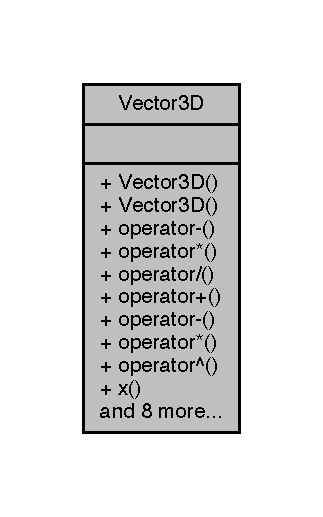
\includegraphics[width=155pt]{doxygen/latex/class_vector3_d__coll__graph}
\end{center}
\end{figure}
\subsection*{Public Member Functions}
\begin{DoxyCompactItemize}
\item 
\hypertarget{class_vector3_d_a9c58f21ac5a280f62067d7f26466ba47}{}\label{class_vector3_d_a9c58f21ac5a280f62067d7f26466ba47} 
{\bfseries Vector3D} (const double x, const double y, const double z)
\item 
\hypertarget{class_vector3_d_a5fc1291699c792e6acd5ea453c47f3f4}{}\label{class_vector3_d_a5fc1291699c792e6acd5ea453c47f3f4} 
\hyperlink{class_vector3_d}{Vector3D} {\bfseries operator-\/} (void) const
\item 
\hypertarget{class_vector3_d_afa1d5717e088826b6dcc0cb35ec836f7}{}\label{class_vector3_d_afa1d5717e088826b6dcc0cb35ec836f7} 
\hyperlink{class_vector3_d}{Vector3D} {\bfseries operator$\ast$} (const double a) const
\item 
\hypertarget{class_vector3_d_a86a2dec32df2740e92e06b651d693c95}{}\label{class_vector3_d_a86a2dec32df2740e92e06b651d693c95} 
\hyperlink{class_vector3_d}{Vector3D} {\bfseries operator/} (const double a) const
\item 
\hypertarget{class_vector3_d_af75a42c25ca6e999f3e7a83d4de105c6}{}\label{class_vector3_d_af75a42c25ca6e999f3e7a83d4de105c6} 
\hyperlink{class_vector3_d}{Vector3D} {\bfseries operator+} (const \hyperlink{class_vector3_d}{Vector3D} \&v) const
\item 
\hypertarget{class_vector3_d_acd7927ced75a36b459200a791e51acad}{}\label{class_vector3_d_acd7927ced75a36b459200a791e51acad} 
\hyperlink{class_vector3_d}{Vector3D} {\bfseries operator-\/} (const \hyperlink{class_vector3_d}{Vector3D} \&v) const
\item 
\hypertarget{class_vector3_d_a307962a6472b58ac85af69ad74c4fd6f}{}\label{class_vector3_d_a307962a6472b58ac85af69ad74c4fd6f} 
double {\bfseries operator$\ast$} (const \hyperlink{class_vector3_d}{Vector3D} \&b) const
\item 
\hypertarget{class_vector3_d_ac6d8d994b5c80eaaed1f033fd7baa627}{}\label{class_vector3_d_ac6d8d994b5c80eaaed1f033fd7baa627} 
\hyperlink{class_vector3_d}{Vector3D} {\bfseries operator$^\wedge$} (const \hyperlink{class_vector3_d}{Vector3D} \&v) const
\item 
\hypertarget{class_vector3_d_ac86d9a556616f4c51fecbaf7d8658ce8}{}\label{class_vector3_d_ac86d9a556616f4c51fecbaf7d8658ce8} 
double {\bfseries x} () const
\item 
\hypertarget{class_vector3_d_a7146d35db2c1bf7606c8290282a423ec}{}\label{class_vector3_d_a7146d35db2c1bf7606c8290282a423ec} 
double {\bfseries y} () const
\item 
\hypertarget{class_vector3_d_af4ae427e82a23af845f804106daed509}{}\label{class_vector3_d_af4ae427e82a23af845f804106daed509} 
double {\bfseries z} () const
\item 
\hypertarget{class_vector3_d_af396bfa140d140d818a97100f7d6a532}{}\label{class_vector3_d_af396bfa140d140d818a97100f7d6a532} 
double {\bfseries dot\+Product} (const \hyperlink{class_vector3_d}{Vector3D} \&v) const
\item 
\hypertarget{class_vector3_d_a15b417a5abd07b8a7403bdb0ac5f95ec}{}\label{class_vector3_d_a15b417a5abd07b8a7403bdb0ac5f95ec} 
\hyperlink{class_vector3_d}{Vector3D} {\bfseries cross\+Product} (const \hyperlink{class_vector3_d}{Vector3D} \&v) const
\item 
\hypertarget{class_vector3_d_a4ddb90e85e10f0f32475725cb966a5ce}{}\label{class_vector3_d_a4ddb90e85e10f0f32475725cb966a5ce} 
double {\bfseries length} () const
\item 
\hypertarget{class_vector3_d_aac87aef508e65eb8ada23346b5e552c3}{}\label{class_vector3_d_aac87aef508e65eb8ada23346b5e552c3} 
\hyperlink{class_vector3_d}{Vector3D} {\bfseries normalized} () const
\item 
\hypertarget{class_vector3_d_a1698a0e33c975b78f0076b51331e6e94}{}\label{class_vector3_d_a1698a0e33c975b78f0076b51331e6e94} 
\hyperlink{class_vector3_d}{Vector3D} {\bfseries rotated\+AboutZ} (const double angle) const
\item 
\hypertarget{class_vector3_d_a5df051b736bdb50b63995442b0816938}{}\label{class_vector3_d_a5df051b736bdb50b63995442b0816938} 
bool {\bfseries is\+Normal} () const
\end{DoxyCompactItemize}


The documentation for this class was generated from the following files\+:\begin{DoxyCompactItemize}
\item 
Raytracer3\+D/\+Raytracer3\+D/Vector3d.\+hpp\item 
Raytracer3\+D/\+Raytracer3\+D/Vector3d.\+cpp\end{DoxyCompactItemize}

%--- End generated contents ---

% Index
\backmatter
\newpage
\phantomsection
\clearemptydoublepage
\addcontentsline{toc}{chapter}{Index}
\printindex

\end{document}
